\documentclass[review]{elsarticle}

\usepackage{lineno,hyperref}
\modulolinenumbers[5]

\journal{Journal of \LaTeX\ Templates}

\usepackage{graphicx}
\usepackage{epsfig}
\usepackage{epstopdf}
%\usepackage{cite}
\usepackage{algorithm}
\usepackage{algpseudocode}
\renewcommand{\algorithmicrequire}{\textbf{Input:}}
\renewcommand{\algorithmicensure}{\textbf{Output:}}
\usepackage{amsmath}
\usepackage{amsfonts}
\usepackage{subfigure}
%\usepackage{subcaption}

%%%%%%%%%%%%%%%%%%%%%%

\begin{document}

\begin{frontmatter}
%\title{ Efficient Prediction for Label Tree-Based Multi-class Classification }
\title{ Reducing Error Propagation for Hierarchical Classification }
%\title{Elsevier \LaTeX\ template\tnoteref{mytitlenote}}
%\tnotetext[mytitlenote]{Fully documented templates are available in the elsarticle package on \href{http://www.ctan.org/tex-archive/macros/latex/contrib/elsarticle}{CTAN}.}
%% Group authors per affiliation:
\author[mymainaddress]{Tien-Dung Mai\corref{cor1}}
\ead{dungmt@uit.edu.vn}
%\fntext[myfootnote]{Corresponding author}

\author[mymainaddress]{Thanh Duc Ngo}
\ead{thanhnd@uit.edu.vn} 

\author[mymainaddress,mysecondaryaddress]{Duy-Dinh Le}
\ead{ledduy@nii.ac.jp}

\author[mymainaddress]{\\Duc Anh Duong}
\ead{ducda@uit.edu.vn}  

\author[mymainaddress]{Kiem Hoang}
\ead{kiemhv@uit.edu.vn}

\author[mysecondaryaddress]{Shin'ichi Satoh}
\ead{satoh@nii.ac.jp} 

\cortext[cor1]{Corresponding author}				
\address[mymainaddress]{University of Information Technology, VNU-HCM, Ho Chi Minh City, Vietnam }
\address[mysecondaryaddress]{National Institute of Informatics, 2-1-2 Hitotsubashi, Chiyoda-ku, Tokyo, Japan}

\begin{abstract}
%Old: A label tree is a computational efficient approach for multi-class classification with a large number of class labels. A main limitation of this approach is a propagating error problem where errors made at a parent node cannot be corrected at its child nodes during traversing the tree for classification.In this paper, we propose a novelty method that use information about scoring-relations among candidate nodes and relations between candidate nodes and their children to reduce this error. Specifically, we first combine the score value returned by a binary classifier of current node and the score values returned by binary classifiers of its child nodes into pseudo feature vectors, and then, we formulate a procedure to select next visited node as an objective function that is learned basing set of pseudo feature vectors on validation set. Experimental results on image benchmark datasets such as Caltech-256, SUN-397 and ILSVRC2010-1K demonstrate the performance of our method.

% ICIP: Hierarchical classification is a computational efficient approach for multi-class classification, given a large number of classes. 
Hierarchical classification is an efficient approach in terms of prediction accuracy at a fraction of the prediction cost .
%ICIP: One of the main challenging problems of this approach is to deal with error propagation. Irrelevant branching decision made at a parent node cannot be corrected at its child nodes in traversing the tree for classification. 
One of the main challenging problems of this approach is to deal with error propagation. Irrelevant branching decision made at a parent node cannot be corrected at its child nodes in traversing the tree for classification. 
This leads to decrease classification accuracy.
%causing a decrease in accuracy
% ICIP: This paper presents a novel approach to reduce branching error at a node by taking its relative relationship into account. Given a parent node on the tree, we model each candidate branch by considering classification response of its child nodes, grandchild nodes and their differences with siblings. A maximum margin classifier is then applied to select the most discriminating candidate. Our proposed approach outperforms related approaches on Caltech-256, SUN-397 and ILSVRC2010-1K.
In this paper we introduce a novel approach to reduce branching error at a node by exploiting its relative relationship. Given a parent node on the tree, 
we develop a new model that allows representing each candidate branch basing on classification response of its child nodes, grandchild nodes and their differences with siblings. 
We then formulate the selecting candidate branch as a maximum-margin problem. By optimizing this problem, we obtain a classifier that can determinate the most discriminating candidate.
Empirical results demonstrate that our proposed approach outperforms related approaches on benchmark datasets such as Caltech-256, SUN-397 and ILSVRC2010-1K.

\end{abstract}
%
\begin{keyword}
Hierarchical classification \sep error propagation \sep node relationship \sep large-scale image classification 
\end{keyword}

\end{frontmatter}

\linenumbers


\section{Introduction}
\label{intro}
%Old: A large-scale multi-class classification is one of interesting challenges. It has received a great interest in several fields such as vision computer vision and machine learning. Because there are many real applications that require a classification with large number of class labels where the popular one-versus-all classifiers-based methods become in-feasible due to the testing cost is linear with the number of classes \cite{DengECCV2010}, \cite{Akata.TPAMI2013}, \cite{ILSVRC15}, \cite{HOSong15PAMI}. 
%ICIP: Multi-class image classification is essential to various applications. One of the challenges is to classify a large number of classes. This makes standard one-versus-all approach impractical since its computational complexity is linear with the number of classes \cite{DengECCV2010}, \cite{Akata.TPAMI2013}, \cite{ILSVRC15}, \cite{HOSong15PAMI}. 

Multi-class image classification is a challenges problem with a large number of classes, dimensions and images. A widely used approach is one-versus-all strategy where an independent classifier is learnt per class. However, the classifying cost might be expensive since all the classifiers would need to be evaluated every time for predicting a given test image. This is impractical when the number of classes is large \cite{DengECCV2010}, \cite{Akata.TPAMI2013}, \cite{ILSVRC15}, \cite{HOSong15PAMI}. 

%ICIP: Recently, several hierarchical classification approaches (i.e. tree-based approaches) \cite{Bengio.NIPS2010}, \cite{Deng.NIPS2011},\cite{WangICME13}, \cite{Liu.CVPR2013.ProbTree}, \cite{Zhu.CVIU2014}, \cite{SunICCV2013} have been proposed to tackle that scalability issue. 
Recently, several hierarchical classification approaches (i.e. tree-based approaches) \cite{Bengio.NIPS2010}, \cite{Deng.NIPS2011},\cite{WangICME13}, \cite{Liu.CVPR2013.ProbTree}, \cite{Zhu.CVIU2014}, \cite{SunICCV2013}, \cite{Babbar.NIPS2013_5082} have been proposed to tackle that scalability issue. 
%ICIP: In these approaches, each node is associated with a subset of class labels and a classifier. The classifier produces a response indicating how relevant a new image or test sample to the class labels of the node. A leaf node associates with only one class. 
The key idea of these approaches is to organize a given set of classes into a hierarchical tree structure in which each node is associated with a subset of class labels and a classifier. The classifier produces a response indicating how relevant a new image or test sample to the class labels of the node. A leaf node associates with only one class. A root node is associated with the entire set of classes.
%ICIP: Classifying a given test sample is achieved by traversing the tree from its root to a leaf node. 
Classifying a given test sample is achieved by traversing the tree from its root until it reaches a leaf node. 
At each visited node, classifiers of their children are applied. The returned scores from the classifiers are then used to determinate the next node to move on.  
% This leads to prediction costs that are sub-linear or even logarithmic if the tree is balanced.
With such top-down traversing procedure, tree-based approaches have a well-known problem - propagation error problem. Errors made at a higher level in the label tree cannot be corrected at later levels \cite{Liu.CVPR2013.ProbTree}, \cite{Zhu.CVIU2014}. 
% ICIP: Standard selection strategy is the highest-response-first strategy i.e. the child node with the highest response is selected (Fig. \ref{fig:Standard}). However, if the nodes or classes of nodes are highly indiscriminate, such selection might result in poor classification accuracy. 
The origination of this error is caused by tree organization. In tree-based model, at each node $v$ of the tree that it has at most $Q$ children per node for branching, a set of class labels $\ell(v)$ of node $v$ are partitioned into $Q$ groups, each group corresponds to a child node, and classifiers of nodes are then learned. Due to the number of class labels $|\ell(v)|$ is often greater than the number of children $Q$, it is difficult to obtain $Q$ groups clearly discriminated. 
Moreover, in the tree building process from training set, to guarantee balanced tree structure for efficiency, an equal number of class labels in each group (or associated with each child node) should be maintained. This leads to highly related classes can be partitioned into different groups. 

As a result, the highest response score of these classifiers is not confident enough to make the correct decision every time. 
%ICIP: A popular selection strategy is the highest-response-first strategy i.e. the child node with the highest response is selected. 
So, only selecting the child node with the highest response score to move on (Fig. \ref{fig:Standard}) - referred as the highest-response-first strategy - might decrease classification accuracy. .

% old: Instead of only relying on the highest predict score to make selecting decision as the existing standard selection method, the relation between scores with others has been recently considered to improve the classification accuracy. 
%ICIP: To overcome above mentioned problems, the relation between scores with others has been recently considered.
To tackle above mentioned problems, the relation between scores with others has been recently considered.
Liu et al. \cite{Liu.CVPR2013.ProbTree} introduced an method that allows visiting nodes with highest score and the second highest score if the difference between them is below a threshold value. 
Although this way is able to improve accuracy, it is not only increasing the classification cost when selecting occur at higher level node, but also difficult to determinate a adaptive global threshold in practical.  
Zhu et al. \cite{Zhu.CVIU2014} proposed an method that concatenates the scores of candidate nodes and of their children into a meta feature vector that is used to select visited node by a multi-class regression. 
However, this method ignores information about their relative difference.

%%--------------------- new Proposal
%In this paper, we address this problem and introduce new
% ICIP: In this work, we study to further extend the effectiveness of using relationship of relative nodes for making precise branching decision. 
In this work, our objective is to further extend the effectiveness of using relationship of relative nodes that is more accurate at branching decision than the highest-response-first based approach and the approach of Zhu et al. \cite{Zhu.CVIU2014}.
%ICI{: Compared to the approach of Zhu et al. \cite{Zhu.CVIU2014}, our approach is different with following extensions. 
Our main contributions are follows:
\begin{itemize}
\item First, we do not only use response scores from classifiers of child nodes and grandchild nodes of the current node. We further extend by also considering their relative differences. Given a parent node on the tree, we model each candidate branch by considering classification response of its child nodes, grandchild nodes and their differences with siblings at different levels (Fig. \ref{fig:Ours}). All of such information is composed into a feature vector representing the candidate branch. 
\item Second, we formulate branching decision making as an optimization problem. By solving the problem, we obtain a maximum margin classifier by which the most discriminating candidate branch can be selected. Additionally, our formulation is closely related to Multiple Instance Learning (MIL). Thus, it can take the advantages of MIL to deal with weakly labeled data in training process.
\end{itemize}
% Exp
We evaluate the approach on several benchmark including Caltech-256, SUN-397 and ILSVRC2010-1K. Experimental results indicated that our proposed approach improve classification accuracy, compared to other related approaches.

\begin{figure*}
\centering
 \subfigure[Presenting the baseline approach which relies on highest-response-first strategy]{
 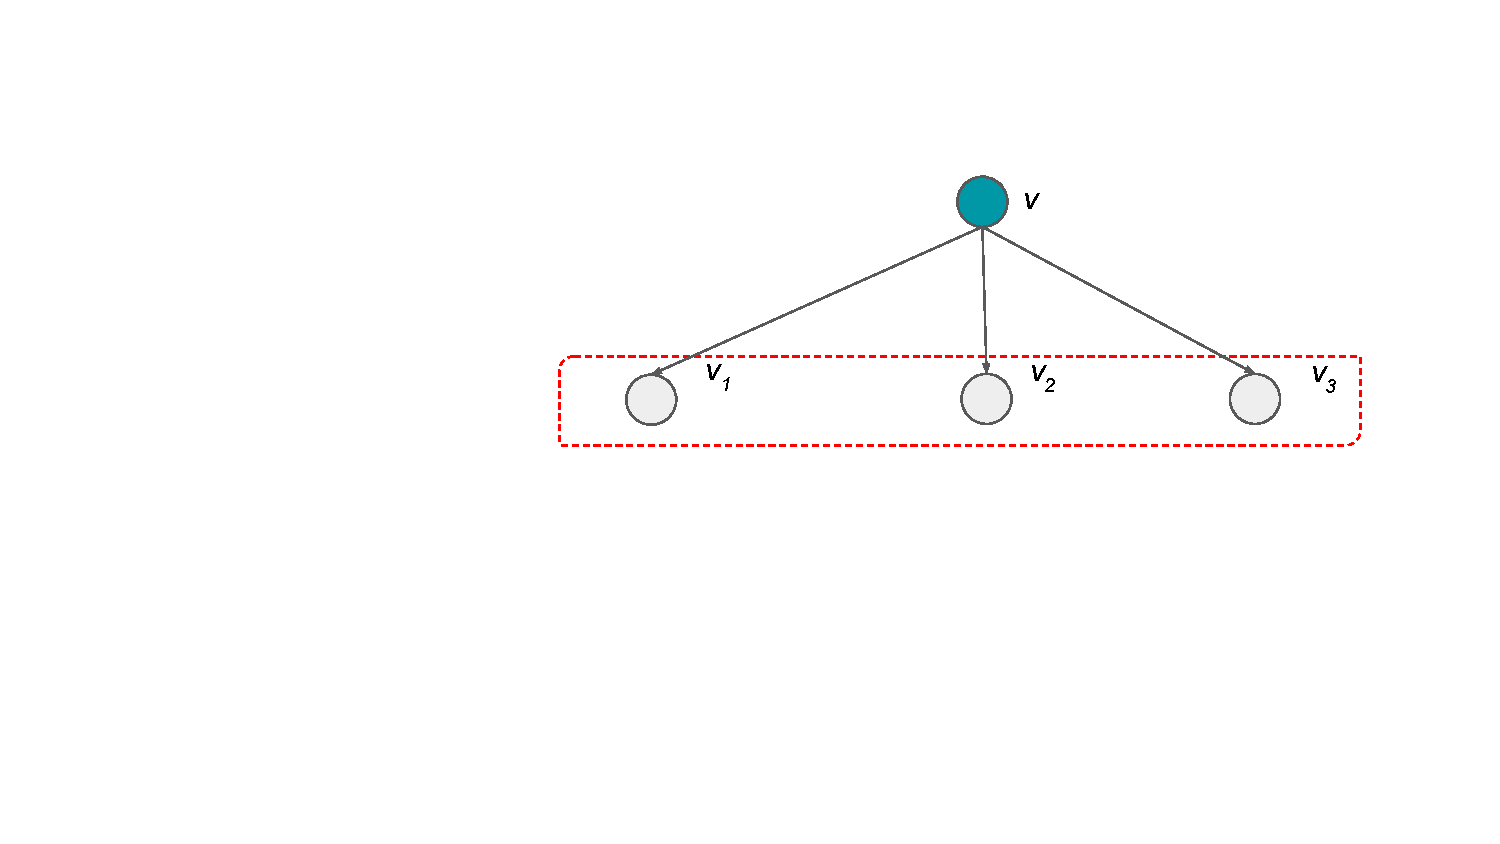
\includegraphics[width=0.80\textwidth]{Fig01a.pdf}
 \label{fig:Standard}
 } \\ %\hspace{0.5em}%
\subfigure[illustrates Zhu et al.'s method  \cite{Zhu.CVIU2014} relying on a meta feature constructed by concatenating the prediction scores of child nodes and grand child nodes.]{
 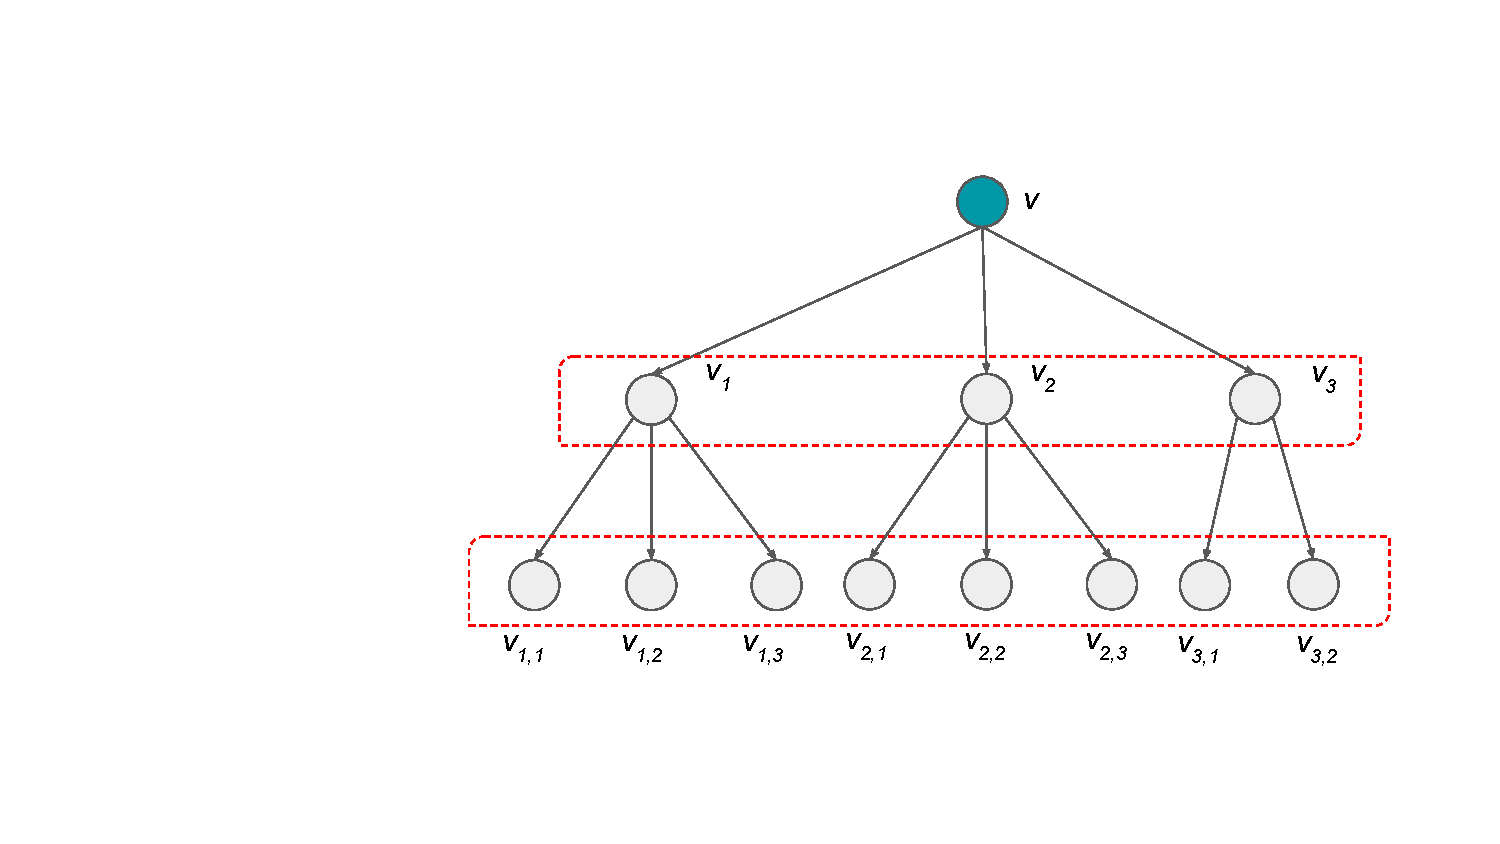
\includegraphics[width=0.82\textwidth]{Fig01b.pdf}
 \label{fig:ER}
 } \\
% \hspace{0.5em}%
\subfigure[Illustrating our proposal. The approach takes into account the relationships between child nodes, grand child nodes and their siblings.]{
 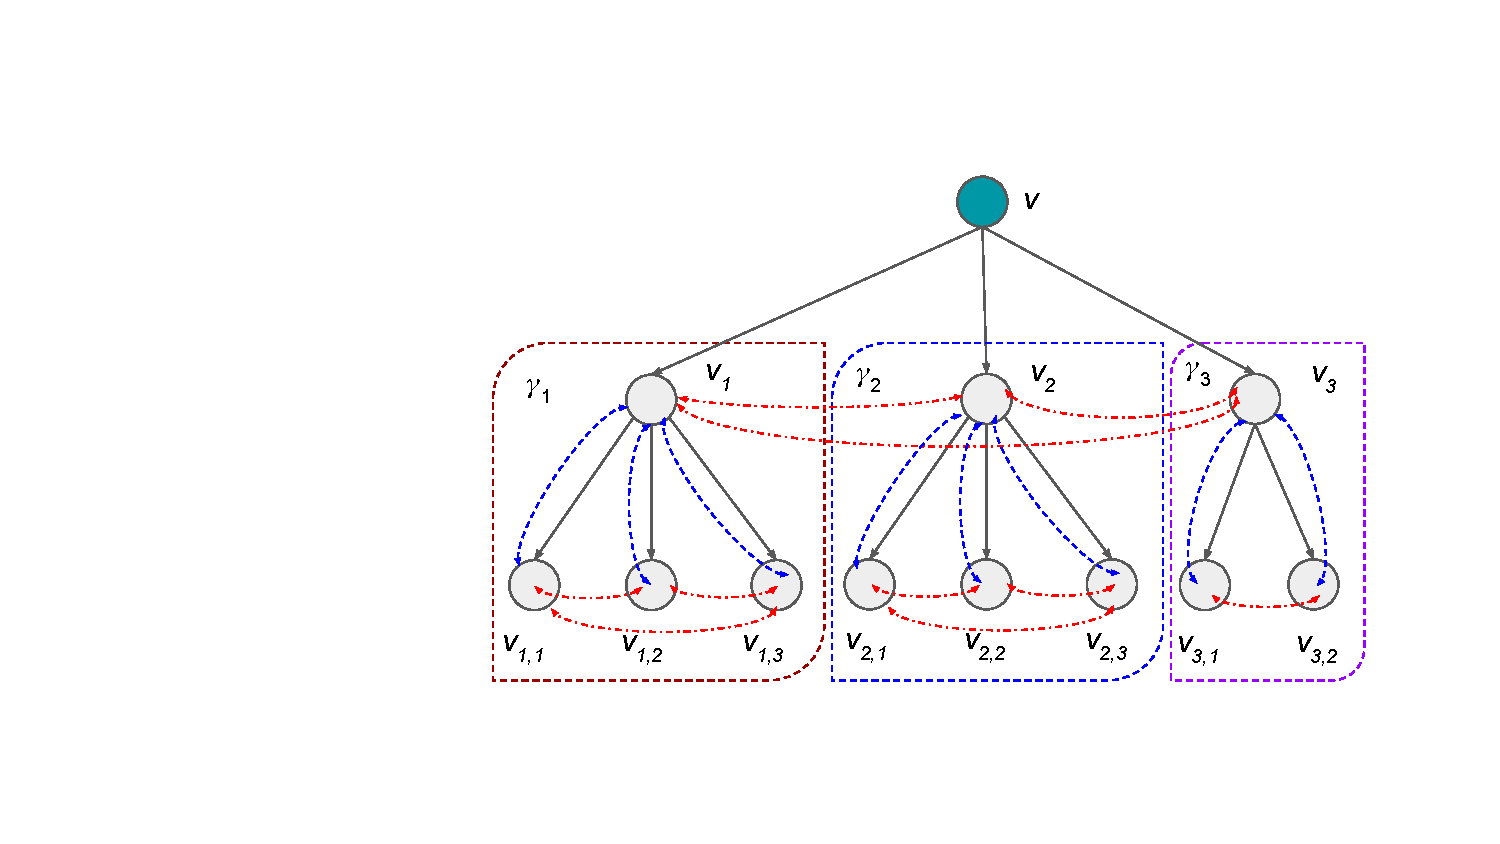
\includegraphics[width=0.82\textwidth]{Fig01c2.pdf}
 \label{fig:Ours}
 } 
\caption{Different approaches to select the next node from the current node $v$}
	\label{fig:SelectNode}
\end{figure*}

%% Paper organization
The rest of the paper is organized as follows. In Section \ref{sec:relatedwork}, related works are presented. In Section \ref{sec:ourmethod}, the proposed method is described. The experimental results are presented in Section \ref{sec:experiments}. Finally, Section \ref{sec:conclusion} concludes the paper.

% =================================

\section{Related work} \label{sec:relatedwork}

A challenge problem in a tree-based approaches is how to use the tree for accurate classification. 
The popular method usually selects the branch or node whose corresponding predict score is highest to follow in the next step. 
In cases where there is ambiguity in the correct node, this selection will reduce the classification accuracy if the wrong node is selected. 

Providing such label trees, avoiding irrelevant branching decision is essential to improve classification accuracy. Beside the highest-response-first strategy, several other approaches introduced recently. 

Sun et al. \cite{SunICCV2013} considered the classification problem as finding the best path in the label tree and proposed a branch-and-bound-like algorithm to efficiently search for the best path. To trade-off between efficiency and accuracy, both the bounds and the classifiers are jointly learned using structured SVM formulation with additional bound constraints.

Wang and Forsyth in \cite{WangICME13} proposed a method that aggregate the probability distribution associated with leaf node of trees in a label forest i.e. an ensemble of label trees. The $(i+1)$-th label tree is constructed by applying Bengio et al. method \cite{Bengio.NIPS2010} with confusion matrix computed for the $i$-th label tree on a validation set. Although this method improved the classification accuracy, the computational cost can be significantly increased with a large number of label trees. 

Liu et al. \cite{Liu.CVPR2013.ProbTree} introduced a method that rises the classification accuracy by performing a limited search over multiple branches of the label tree. A choice is made by comparing the difference in scores between the highest-scoring and the second highest-scoring branch. If this difference is below a threshold, both branches are traversed. Although, the classification accuracy is increased as the classification process explores more branches, the computational efficiency is decreased and the value of threshold is manually tuned to balance the accuracy and efficiency trade-off. However, this indicates that the relationship among nodes can help to improve classification accuracy. 

In \cite{Zhu.CVIU2014}, Zhu et al. has found that the classification error may be reduced by using the semantic and contextual relationship among candidate nodes and their children to recover the responses of unreliable classifiers of the candidate nodes. They simply concatenated the scores of candidate nodes and of their children into a meta feature vector that is used to predict candidate node by using multi-class regression (Fig. \ref{fig:ER}).

% MIL ??


%\section{Method Overview} \label{sec:ourmethod}
\section{Our Approach} \label{sec:ourmethod}

In contrast with prior research, we investigate a novel technique to perform effective selection which best branch to follow. 
In this section, we first describe a method to represent the relationship between candidate nodes and of its children as sets of feature vectors in subsection \ref{sec:relationships} , and then the node selection is formulated as an optimize problem in subsection \ref{sec:formulation}, and finally the classification for new testing images is described in subsection \ref{sec:classification}
% Relationship
\subsection{Representing Node Relationships} \label{sec:relationships}
In this work, we take into account relationships between child nodes and grandchild nodes together with their siblings, instead of simply concatenating response scores from classifiers at nodes as in \cite{Zhu.CVIU2014}. A candidate branch from the current node is represented by using: i) the prediction score from classifier of its child node along the branch; ii) the prediction score from classifier of its grandchild node along the branch; ii) differences in prediction scores between the child node and the grandchild node with other sibling nodes at the same level.

Specifically, let $p_v(x)$ be a prediction score of image $x$ returned by the classifier of node $v$, and $\ell(v)$ denotes the set of class labels that belong to node $v$. $\psi(v)$ is the set of children of node $v$, $v_i \in \psi(v)$ indicates the $i$-th child of node $v$  and $v_{i,j} \in \psi(v_i)$ indicates the $j$-th child of node $v_i$.

Suppose that we are considering the current node $v$, the task is to select one of its child nodes to visit next. Noted that we select one child node here for simplification. In general, more than one node can be selected. Let $\rho_{v_i}(x) \in \mathbb{R}^{|\psi(v)|}$ is a vector composed by the prediction score $p_{v_i}(x)$ and the difference between $p_{v_i}(x)$ and those of siblings of $v_i$. It can be represented as follows:


\begin{multline}
\rho_{v_i}(x) = [p_{v_i}(x), p_{v_i}(x)-p_{v_1}(x), .. , p_{v_i}(x) - p_{v_{|\psi(v)|}}(x)] 
\end{multline}
Then, a feature vector that describes the relation between a node $v$ with its child node, its grandchild nodes and differences to their siblings can be formulated as:
\begin{align}
\varphi_{i,j}(x) = [ \rho_{v_i}(x) , \quad  \rho_{v_{i,j}}(x) ]
\end{align}
Noted that $\varphi_{i,j}(x)$ also represents a candidate branch which traverses through $v_i$ and $v_{i,j}$.


\subsection{Problem Formulation} \label{sec:formulation}

For each node $v_i$, we have the set of candidate branches go through $v_i$ is:
\begin{align}
 \gamma_{v_i}(x) = \{\varphi_{i,1}(x), \varphi_{i,2}(x), .., \varphi_{i,|\psi(v_i)|}(x) \}
\end{align}
Accordingly, the set of all possible branches from $v$ is $\gamma_{v_i}(x),\forall v_{i,j} \in \psi(v_i)$.
Then, the problem of selecting the next node to move on becomes selecting suitable $v_{i}$. We formulate the problem as a max margin optimization problem.

Assuming we are given an image $x$ with label $y$. A candidate branch represented by a feature vector $\varphi_{i,j}(x)$ is labeled positive if the label $y \in \ell(v_i)$ and $y \in \ell(v_{i,j})$. Otherwise, the branch is labeled negative.

A set $\gamma_{v_i}(x)$ representing all possible branches go through $v_i$ is labeled positive if it contains at least one positive branch. It is labeled negative if all of its branches are negative. Selecting a candidate node $v_i$ to follow is equivalent to finding a corresponding positive set $\gamma_{v_i}(x)$.  

Using images having ground-truth class labels belong to $\ell(v)$ of a node $v$, we can obtain positive sets and negative sets. We use $\Gamma_{v}^{+} $ to denote the set of all positive sets $\gamma_{v_i}(.)$ and $\Gamma_{v}^{-} $ to denote the set of all negative sets $\gamma_{v_i}(.)$.

We then find a margin function with parameters $(w, b)$ to maximize the margin between positive set $\Gamma_{v}^{+} $ and negative set $\Gamma_{v}^{-} $ by solving the following optimization problem:
\begin{equation}
\arg\min_{w_{v}, b, \{\xi_i\}} \frac{1}{2} \|w_{v}\|^2 + C \sum_{i} \xi_i  
\end{equation}
subject to 
\begin{equation}
\max_{\gamma \in \Gamma_{v}^{+} } (w_{v}^T \cdot \gamma + b) \ge 1 - \xi_i, ~~~~ \forall i=1,...,|\Gamma_{v}^{+}| , \xi_i \ge 0
\end{equation}
\begin{equation}
\max_{\gamma \in \Gamma_{v}^{-} } (w_{v}^T \cdot \gamma + b) \leq -1 + \xi_j, ~~~~ \forall j=1,...,|\Gamma_{v}^{-}| , \xi_j \ge 0
\end{equation}
where $C$ is a constant, $\{\xi_i\}$ are non-negative slack variables.

This problem is solved as in \cite{AndrewsNIPS2002}, we obtain a classifier that can be used to determinate a candidate node $v_i$ to follow in the next step.

\subsection{Classification Stage} \label{sec:classification}

Given a new testing image $x$, classification are performed by traversing the tree from its root to a leaf node. At each node $v$ along the path, we first obtain a set  $\Gamma_{v}^x$. $\Gamma_{v}^x$ includes $|\psi(v)|$ sets of candidate branches go through $v_i, v_i \in \psi(v)$.  
\begin{align}
\Gamma_{v}^x = \{ \gamma_{v_1}(x),.., \gamma_{v_{|\psi(v)|}}(x) \} \label{eq:Gammax}
\end{align}

We then select node $v_i$ whose $\tilde{\gamma}$ yielding the largest.
\begin{equation}
\tilde{\gamma} = \arg\max_{\gamma \in \Gamma_{v}^x} (w_{v}^T \cdot \gamma + b) \label{eq:test}
\end{equation}

We summarize the algorithm for classification in Algorithm \ref{alg_labeltree_predict} as follows.
\begin{algorithm}
  	\caption {Classification } \label{alg_labeltree_predict}
  	\begin{algorithmic}[1]
  		\show\LOOP
  		\Require {The label tree $T=(V,E)$ with the root node $r$ and  a testing image $x$}
  		
  		\Ensure   Class label of $x$.
		\State $v \gets r$
		\While { $\sigma(v) \neq \emptyset$ }
			\State Obtain  $\Gamma_{v}^x$ by equation (\ref{eq:Gammax})
	    	\State $v \gets v_i$ correspond to $\tilde{\gamma}$ obtained by equation (\ref{eq:test}).		
    	\EndWhile
    	\State \textbf{return} { ${l}(v)$}
	\end{algorithmic}
\end{algorithm}


\section{Experiments} \label{sec:experiments}
%This section describes experiments on several datasets for large-scale image classification.
\subsection{Datasets}
We conducted experiments on several benchmark which are widely used to evaluate large-scale image classification approaches.  

\begin{itemize}
\item \textbf{Caltech-256} dataset \cite{GriffinCaltech256}. This is a dataset for multi-class object classification. There are 29,780 images of 256 object classes. Each image is assigned to a single class label, each class contains at least 80 images. 

\item \textbf{SUN-397} dataset \cite{SUN2010}. This dataset is a subset of the SUN dataset. It is selected from 908 scene classes for a scene classification. There are 108,754 images of 397 classes with at least 100 images per class.

\item \textbf{ILSVRC2010-1K} dataset \cite{ILSVRC15}. This is a challenging dataset, especially for large-scale image classification. The dataset includes 1,461,406 images of 1,000 classes. Each class has at least 668 images.
\end{itemize}

The dataset is divided into a training set, a validation set and a test set. 
The training set is used to learn classifier at each non-leaf node of tree. 
The validation set is used to train maximum margin classifier (proposed approach), multi-class regression ( described in \cite{Zhu.CVIU2014}), and to obtain confusion matrix used for building tree structure (described in \cite{Bengio.NIPS2010}). 
 
In the case of ILSVRC2010-1K, we use the provided validation set and test set. We randomly pick 300 images per category for training. 

With Caltech-256 and SUN-397, the images of each category are randomly split to 50\% for training, 25\% for validation and remaining images for testing. 
To obtain stable experimental results, the random split was performed 5 times. And then, we reported the average classification performance with the corresponding standard deviation. 
 
\textbf{Feature:} We follow the widely used feature settings as in \cite{Deng.NIPS2011}, \cite{Liu.CVPR2013.ProbTree}. In particular, each image is represented using Locality-constrained Linear Coding (LLC) described in \cite{Wang.CVPR2010} with densely sampled SIFT features extracted by VLFeat toolbox \cite{Vedaldi10vlfeat}. A codebook with 10,000 visual words is used together with two-level Spatial Pyramid Matching (SPM) \cite{Lazebnik.CVPR2006} with $1 \times 1$ and $2 \times 2$ grids. Consequently, the number of dimensions of each feature vector is 50,000.

%\item \textbf{CNN feature.} We consider using the the state-of-the-art deep visual feature CNN \cite{ChatfieldBMVC14} that is a variation of deep convolutional neural network (CNN) feature \cite{KrizhevskyNIPS12}. It comprises 5 convolutional layers, and 3 fully-connected layers. The number of dimension of the final layer is 4,096. This resulted in a feature vector with 4,096 dimensions for image representation.

\subsection{Experimental Setting} 
\subsubsection{The Tree Configures}
In order to show the performance of our proposed approach, we conducted experiments with three following configurations:
\begin{itemize}
\item The pre-defined tree. This is a tree structure that created manually basing on semantic relations or the hierarchical structure of WordNet. 

\item The label tree. We employ the approach of Bengio et al. \cite{Bengio.NIPS2010} for tree construction. Specifically, binary one-versus-all classifiers firstly are trained form training set. These classifiers are applied on a validation set to obtain a confusion matrix. A spectral clustering algorithm \cite{ng2002spectral} is then applied recursively to partition the label sets of a current node into disjoint groups of classes. Each group associates to one child node of the current node. Since spectral clustering penalizes unbalanced partitions, the resulting tree structure can be unbalanced. The tree is denoted by $T_Q$ and it has at most $Q$ children per node for branching.

\item The balanced label tree. We consider a case of balanced label tree \cite{MaiICIAP15} to achieve the logarithmic run-time. The tree structure is built by jointly optimizing the balance constraint and the confusion constraint during learning. The balanced tree is denoted by $T_{Q,H}$ that it has at most $Q$ children per node for branching and the maximum height is $H$.

\end{itemize}

\subsubsection{Baseline approaches}
We compare the performance of proposed approach with to closely related approaches.
\begin{itemize}
\item Baseline. This is the popular approach which relies on the highest-response-first strategy for selecting a next branch.
\item ER-SHC \cite{Zhu.CVIU2014}. We directly compare to this approach since it is the most related approach to our proposal. Both approaches aim at improving classification accuracy by employing relationships of nodes. This direct comparison is to realize the effectiveness of utilizing more information of node relationships into branch selection and max margin formulation.
% (referred to ER-SHC, denoted as ER-SHC)
\end{itemize}

\subsection{Results and Discussions}

\subsubsection{Results on The Predefined Tree}
Table \ref{tbl:PreTree} shows the experimental results on the pre-defined tree of ILSVRC2010-1K, SUN-397, and Caltech-256, respectively.
Each column of table is associated with dataset, and each row shows the performance of methods. As we can see, the performance of our proposed method is better than others.

\begin{table}
\caption{Performances of methods on predefined tree using SIFT-LLC-SPM feature.}  
\label{tbl:PreTree} 
\centering
\begin{tabular}{llll}
\hline\noalign{\smallskip}
Methods  & \multicolumn{1}{c}{ImageNet-1K} & \multicolumn{1}{c}{SUN-397} & \multicolumn{1}{c}{Caltech- 256} \\
\noalign{\smallskip}\hline\hline\noalign{\smallskip}
Standard 	 				& x $\pm$x & 37.39 $\pm$0.45 & 35.45 $\pm$0.34 \\
ER-SHC \cite{Zhu.CVIU2014} 	& x $\pm$x & 39.57 $\pm$0.48 & 36.43 $\pm$0.34 \\
Ours     				    & x $\pm$x & 41.34 $\pm$0.32 & 36.85 $\pm$0.28 \\
%Ours(+)     				& x $\pm$1.92 & 42.41 $\pm$0.07 & 37.95 $\pm$0.18 \\
\noalign{\smallskip}\hline\noalign{\smallskip}
\end{tabular}
\end{table}

\subsubsection{Results on The Label Tree}

%Comparing the performance of the different strategies for selecting following node on ILSVRC2010-1K dataset are illustrated in Table \ref{tbl:ImageNet1KSIFT}. As can be seen, for all types of tree configurations, our method achieves significantly better classification accuracy with around 3\% than others. Meanwhile, the accuracy of approach proposed by Zhu et al.\cite{Zhu.CVIU2014} is only more slightly better than the highest score-based approach.
The performance of the evaluated approaches on ILSVRC2010-1K is reported in Table \ref{tbl:ImageNet1KSIFT}. For all tree configurations, our proposed approach achieved significant accuracy improvement over other approaches. The approach of Zhu et al. performed slightly better than the baseline approach on this dataset. A consistent observation is that accuracy of all approaches drops as the maximum number of branches $Q$ of the tree $T_Q$ is reduced. This can be explained by the fact that the smaller $Q$ is the larger number of classes are partitioned into the same group (or branch). It might cause groups more confused; thus, makes precise prediction more challenging.

Furthermore, as $Q$ is decreased, the tree becomes higher. It results in higher chance of choosing an irrelevant branch when traversing. Besides, the accuracy gap between relationship based approaches (i.e. ours and ER-SHC) and the baseline approach is narrowed as $Q$ decreases, since we have less information from nodes for branching decision.

Experimental results on Caltech-256 and SUN-397 are presented in \ref{tbl:Caltech256SIFT} and Table \ref{tbl:SUN397SIFT} respectively. On SUN-397, our approach improve 2\% accuracy over the approach by Zhu et al. \cite{Zhu.CVIU2014} and 3\% accuracy over the Baseline approach. Similarly, our approach outperformed other approaches on Caltech-256, except with $T_2$. With this tree, the feature vector representing each candidate branch is generated with very limited amount of information from nodes. As result, the max margin classifier cannot produce precise selection.


%% -----------------------------------------------------------------------------
% Table ImageNet1K
\begin{table}
\caption{Performance of the evaluated approaches on ILSVRC2010-1K with different tree configurations. The tree is built by Bengio et al.'s method \cite{Bengio.NIPS2010} using SIFT-LLC-SPM feature.}  
\label{tbl:ImageNet1KSIFT} 
\centering
\begin{tabular}{lllll}
\hline\noalign{\smallskip}
Methods  & \multicolumn{1}{c}{$T_{32}$} & \multicolumn{1}{c}{$T_{10}$} & \multicolumn{1}{c}{$T_{6}$} &		\multicolumn{1}{c}{$T_{4}$} \\
\noalign{\smallskip}\hline\hline\noalign{\smallskip}
Baseline 	 				& 7.32 $\pm$0	&	6.01 $\pm$0	&	5.52 $\pm$0	&	5.12 $\pm$0	\\
ER-SHC \cite{Zhu.CVIU2014} 	& 7.70 $\pm$0	&	5.70 $\pm$0	&	5.12 $\pm$0	&	4.66 $\pm$0	\\
Ours	     & \textbf{12.68 $\pm$0}&	\textbf{8.48 $\pm$0}&	\textbf{6.76 $\pm$0}&	\textbf{6.04 $\pm$0}\\
\noalign{\smallskip}\hline\noalign{\smallskip}
\end{tabular}
\end{table}

%% -----------------------------------------------------------------------------

% Table ImageNet1K
\begin{table}
\caption{Performances of methods on ILSVRC2010-1K on tree configurations built by Mai et al.'s method \cite{MaiICIAP15} using SIFT-LLC-SPM feature.}  
\label{tbl:ImageNet1KSIFT.ICIAP} 
\centering
\label{tbl:ImageNet1K} 

\begin{tabular}{lllll}
\hline\noalign{\smallskip}
Methods  & \multicolumn{1}{c}{$T_{32,2}$} & \multicolumn{1}{c}{$T_{10,3}$} & \multicolumn{1}{c}{$T_{6,4}$} &		\multicolumn{1}{c}{$T_{4,5}$} \\
\noalign{\smallskip}\hline\hline\noalign{\smallskip}

Baseline \cite{MaiICIAP15} 	 & 14.07 $\pm$0  & 12.89 $\pm$0  & 12.61 $\pm$0 & 12.20 $\pm$0 \\
ER-SHC \cite{Zhu.CVIU2014}   & 15.95 $\pm$0  & 13.37 $\pm$0  & 12.27 $\pm$0 & 11.97 $\pm$0\\
Ours	     &  \textbf{20.91 $\pm$0} & \textbf{16.13 $\pm$0} & \textbf{14.36 $\pm$0} & \textbf{13.96 $\pm$0} \\

\noalign{\smallskip}\hline\noalign{\smallskip}
\end{tabular}
\end{table}

%% -----------------------------------------------------------------------------
% Table SUN-397
\begin{table*}
\caption{Performance of the evaluated approaches on SUN-397 with different tree configurations. The tree is built by Bengio et al.'s method \cite{Bengio.NIPS2010} using SIFT-LLC-SPM feature.}  
\label{tbl:SUN397SIFT}
\centering
\begin{tabular}{lllll}
\hline\noalign{\smallskip}
Methods  & \multicolumn{1}{c}{$T_{20}$} & \multicolumn{1}{c}{$T_{8}$} & \multicolumn{1}{c}{$T_{5}$} &		\multicolumn{1}{c}{$T_{4}$} \\
\noalign{\smallskip}\hline\hline\noalign{\smallskip}
Baseline 	 				& 30.42 $\pm$0.79 & 24.07 $\pm$0.96 & 23.11 $\pm$0.72 & 21.33 $\pm$0.34 \\
ER-SHC \cite{Zhu.CVIU2014} 	& 30.63 $\pm$0.78 & 24.35 $\pm$1.36 & 23.73 $\pm$0.62 & 21.77 $\pm$0.42 \\

Ours             &  \textbf{34.39} $\pm$0.57 & \textbf{28.21} $\pm$1.21 & \textbf{25.95} $\pm$0.60 & \textbf{23.71} $\pm$0.28 \\
\noalign{\smallskip}\hline\noalign{\smallskip}
\end{tabular}
\end{table*}



%% -----------------------------------------------------------------------------
% Table Caltech256
\begin{table*}
\caption{Performance of the evaluated approaches on Caltech-256 with different tree configurations. The tree is built by Bengio et al.'s method \cite{Bengio.NIPS2010} using SIFT-LLC-SPM feature.}  
\label{tbl:Caltech256SIFT} 
\centering
\begin{tabular}{lllll}
\hline\noalign{\smallskip}
Methods  & \multicolumn{1}{c}{$T_{16}$} & \multicolumn{1}{c}{$T_{7}$} & \multicolumn{1}{c}{$T_{4}$} &		\multicolumn{1}{c}{$T_{2}$}  \\
\noalign{\smallskip}\hline\hline\noalign{\smallskip}
Baseline 	 				& 31.55 $\pm$0.43 & 27.48 $\pm$0.52 & 24.64 $\pm$0.24 & 22.60 $\pm$0.48 \\
ER-SHC \cite{Zhu.CVIU2014} 	& 31.15 $\pm$0.77 & 27.43 $\pm$0.31 & 24.95 $\pm$0.23 & \textbf{22.63} $\pm$0.56 \\

Ours             &  \textbf{37.08} $\pm$0.27 & \textbf{29.32} $\pm$0.52 & \textbf{26.45} $\pm$0.48 & 22.26 $\pm$0.15 \\
\noalign{\smallskip}\hline\noalign{\smallskip}
\end{tabular}
\end{table*}

\subsubsection{Results on The Balanced Tree}
The classification performance for different balanced tree configures on ImageNet-1K, SUN-379, and Caltech-256 are presented Table \ref{tbl:ImageNet1KSIFT.ICIAP}, Table \ref{tbl:SUN397SIFT.ICIAP}, and Table \ref{tbl:Caltech256SIFT.ICIAP}, respectively. 
It can be seen that the our proposed results are better performance than others.
 
%------------------------------------------------------------------------------
% Table SUN-397
\begin{table}
\caption{Performances of methods on SUN-397 on tree configurations built by Mai et al.'s method \cite{MaiICIAP15} using SIFT-LLC-SPM feature.}  
\label{tbl:SUN397SIFT.ICIAP}
\centering
\begin{tabular}{lllll}
\hline\noalign{\smallskip}
Methods  & \multicolumn{1}{c}{$T_{20,2}$} & \multicolumn{1}{c}{$T_{8,3}$} & \multicolumn{1}{c}{$T_{5,4}$} &		\multicolumn{1}{c}{$T_{4,5}$} \\
\noalign{\smallskip}\hline\hline\noalign{\smallskip}
Baseline \cite{MaiICIAP15} 	&  38.49 $\pm$0.75  & 35.94 $\pm$0.89 & 33.90 $\pm$0.52 & 32.94 $\pm$0.70 \\
ER-SHC \cite{Zhu.CVIU2014} 	&  40.72 $\pm$0.01  & 37.05 $\pm$0.11 & 34.99 $\pm$0.44 & 33.87 $\pm$0.12 \\
Ours             &    \textbf{43.04 $\pm$0.01} & \textbf{38.86 $\pm$0.11} & \textbf{35.76 $\pm$0.44} & \textbf{34.05 $\pm$0.12} \\
\noalign{\smallskip}\hline\noalign{\smallskip}

\end{tabular}
\end{table}

% Figure SUN397_Acc
%\begin{figure}
%\centering
% \includegraphics[width=0.75\textwidth]{SUN397_Acc_kchi2.eps}
%\caption{Comparison the performance of the different strategies for selecting the node to follow on SUN-397 dataset}
%\label{fig:SUN397_Acc}
%\end{figure}

%------------------------------------------------------------------------------


% Table Caltech256
\begin{table}
\caption{Performances of methods on Caltech-256 on tree configurations built by Mai et al.'s method \cite{MaiICIAP15} using SIFT-LLC-SPM feature.}  
\label{tbl:Caltech256SIFT.ICIAP} 
\centering
\begin{tabular}{lllll}
\hline\noalign{\smallskip}
Methods  & \multicolumn{1}{c}{$T_{16,2}$} & \multicolumn{1}{c}{$T_{7,3}$} & \multicolumn{1}{c}{$T_{4,4}$} &		\multicolumn{1}{c}{$T_{2,8}$}  \\
\noalign{\smallskip}\hline\hline\noalign{\smallskip}

Baseline \cite{MaiICIAP15} 	 &  38.95  $\pm$0.43  & 35.22 $\pm$0.52 & 33.18 $\pm$0.24 & 29.15 $\pm$0.48 \\

ER-SHC \cite{Zhu.CVIU2014} 	 &  39.10  $\pm$0.48  & 35.49 $\pm$0.68 & 33.42 $\pm$0.60 & \textbf{29.21 $\pm$0.46} \\
			
Ours             &    \textbf{43.53 $\pm$0.46}  & \textbf{36.54 $\pm$0.20} & \textbf{34.42 $\pm$0.39}  & 28.50 $\pm$0.37 \\
			
\noalign{\smallskip}\hline\noalign{\smallskip}
\end{tabular}
\end{table}

\subsubsection{Experiments on Deep Feature}

We carried out additional experiments on Caltech-256 using the the state-of-the-art deep visual VGG-VERYDEEP-16 feature \cite{ChatfieldBMVC14}. Each image is represented by a feature vector with 4,096 dimensions.

Experimental results with the balanced tree \cite{MaiICIAP15} are showed in Table~\ref{tbl:Caltech256CNN.ICIAP}. As you seen, that the accuracy of the proposed method is higher than that of the others. 

%% -----------------------------------------------------------------------------
% Table Caltech256
\begin{table}
\caption{Performances of methods on Caltech-256 on tree configurations built by Mai et al.'s method \cite{MaiICIAP15} using VGG-VERYDEEP-16 feature.}  
\label{tbl:Caltech256CNN.ICIAP} 
\centering
\begin{tabular}{lllll}
\hline\noalign{\smallskip}
Methods  & \multicolumn{1}{c}{$T_{16,2}$} & \multicolumn{1}{c}{$T_{7,3}$} & \multicolumn{1}{c}{$T_{4,4}$} &		\multicolumn{1}{c}{$T_{2,8}$}  \\
\noalign{\smallskip}\hline\hline\noalign{\smallskip}
Baseline \cite{MaiICIAP15} 	 & 72.83 $\pm$0.45  & 69.60  $\pm$0.65 & 68.38 $\pm$0.25 & \textbf{65.89 $\pm$0.54} \\
ER-SHC \cite{Zhu.CVIU2014} 	 & 73.77 $\pm$0.32  & 71.03  $\pm$0.48 & 68.97 $\pm$0.24 & 65.83 $\pm$0.37 \\

Ours             &\textbf{75.18 $\pm$1.09}  & \textbf{71.42 $\pm$0.75} & \textbf{69.05 $\pm$0.28} & 64.94 $\pm$0.54 \\
			
\noalign{\smallskip}\hline
OvA			& \multicolumn{1}{ c }{79.23 $\pm$ 0.42 } 	&  \multicolumn{3}{ c }{}		\\ 
\noalign{\smallskip}\hline\noalign{\smallskip}
\end{tabular}
\end{table}


\subsubsection{Discussions}
\begin{itemize}
\item Compexity of proposed approach: higher than Baseline, same with \cite{Zhu.CVIU2014}. Accuracy is higher than.
\item Effecting of $Q$ and Accuracy ( Fig.\ref{fig:ImageNet1K_Acc_Q})
\end{itemize}

\begin{figure}
\centering
 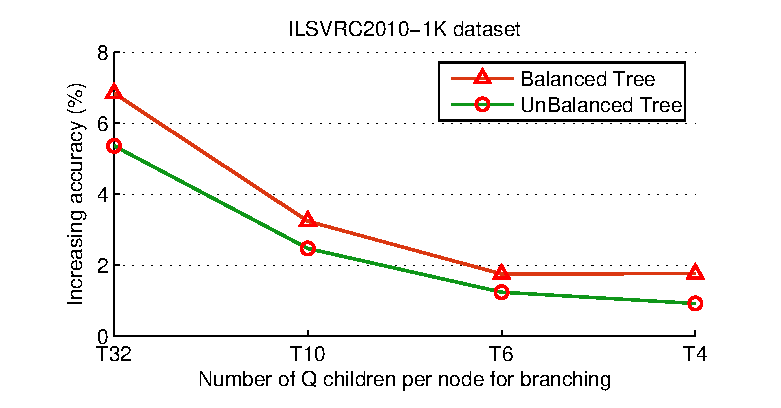
\includegraphics[width=0.75\textwidth]{ImageNet1K_Acc_Q.eps}
\caption{Effecting of $Q$ and Accuracy on ILSVRC2010-1K dataset}
\label{fig:ImageNet1K_Acc_Q}
\end{figure}


% Figure Caltech256_Acc
%\begin{figure}
%\centering
% \includegraphics[width=0.75\textwidth]{Caltech256_Acc_SIFT.eps}
%\caption{Comparison the performance of the different strategies for selecting the node to follow on Caltech-256 dataset}
%\label{fig:Caltech256_Acc}
%\end{figure}
 
\section{Conclusion and Future Work}  \label{sec:conclusion}
%In this paper, we to reduce propagation error in classification, we proposed a node candidate selection approach basing on relation among node candidates and between a node candidate and their children. Our method has been tested on the Caltech-256, SUN-397 and ILSVRC2010-1K benchmark datasets. The experimental results shows that our proposed approach significantly improve classification accuracy comparison to other approaches. 
In this paper, we introduced an approach to reduce propagation error in hierarchical classification by utilizing relationships of nodes. First, given a parent node on the tree, we model each candidate branch by considering classification response of its child nodes, grandchild nodes and their differences with siblings at different levels. Second, we formulate branching decision making as an optimization problem. Experiments on several benchmarks indicated that the proposal help to improve classification accuracy, compared to related approaches.


%\begin{acknowledgements}
%If you'd like to thank anyone, place your comments here
%and remove the percent signs.
%\end{acknowledgements}

%%%%%%%%%%%%%%%%%%%%%%%
%% Elsevier bibliography styles
%%%%%%%%%%%%%%%%%%%%%%%
%% To change the style, put a % in front of the second line of the current style and
%% remove the % from the second line of the style you would like to use.
%%%%%%%%%%%%%%%%%%%%%%%

%% Numbered
%\bibliographystyle{model1-num-names}

%% Numbered without titles
%\bibliographystyle{model1a-num-names}

%% Harvard
%\bibliographystyle{model2-names.bst}\biboptions{authoryear}

%% Vancouver numbered
%\usepackage{numcompress}\bibliographystyle{model3-num-names}

%% Vancouver name/year
%\usepackage{numcompress}\bibliographystyle{model4-names}\biboptions{authoryear}

%% APA style
%\bibliographystyle{model5-names}\biboptions{authoryear}

%% AMA style
%\usepackage{numcompress}\bibliographystyle{model6-num-names}

%% `Elsevier LaTeX' style
\bibliographystyle{elsarticle-num}
\biboptions{sort&compress}


\bibliography{elsarticle-dungmt_mil}

\end{document}
